% The code is quite messy !!!

\documentclass[tikz,border=10pt]{standalone}

\begin{document}

    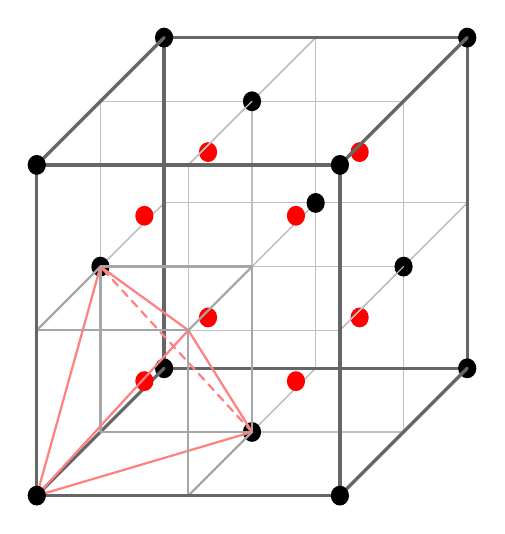
\begin{tikzpicture}[scale=3.5, x={(1.1,0)}, y={(0,1.2)}, z={(0, 0, 1.2)}, line join=round, line cap=round]

    % site tetra arriere
    \foreach \x/\y/\z in {0.25/0.25/0.25, 0.25/0.75/0.25, 0.75/0.25/0.25, 0.75/0.75/0.25} {
        \fill[red] (\x,\y,\z) circle (0.03); % Tetrahedral sites
    }

    % Edges of the small cubes (a/2)
    \foreach \x in {0, 0.5, 1} {
        \foreach \y in {0, 0.5, 1} {
            \foreach \z in {0, 0.5, 1} {
                % Draw edges of each small cube
                \draw[lightgray, thin] (\x,\y,0) -- (\x,\y,1); % vertical edges
                \draw[lightgray, thin] (\x,0,\z) -- (\x,1,\z); % edges parallel to y-axis
                \draw[lightgray, thin] (0,\y,\z) -- (1,\y,\z); % edges parallel to x-axis
            }
        }
    }

    % Cube edges (main cube)
    \draw[black!60, very thick] (0,0,0) -- (1,0,0) -- (1,1,0) -- (0,1,0) -- cycle; % face arriere
    % Vertices of the main cube (face arriere)
    \foreach \x/\y/\z in {0/0/0, 1/0/0, 1/1/0, 0/1/0, 0.5/0.5/0, 0/0.5/0.5, 0.5/0/0.5} {
        \fill[black] (\x,\y,\z) circle (0.03);
    }
    % cube edge
    \draw[black!60, very thick] (0,0,0) -- (0,0,1);
    \draw[black!60, very thick] (1,0,0) -- (1,0,1);
    \draw[black!60, very thick] (1,1,0) -- (1,1,1);
    \draw[black!60, very thick] (0,1,0) -- (0,1,1);

    % site tetra avant
    \foreach \x/\y/\z in {0.25/0.25/0.75, 0.25/0.75/0.75, 0.75/0.25/0.75, 0.75/0.75/0.75} {
        \fill[red] (\x,\y,\z) circle (0.03);
    }
    %cube ou ya le tetraedre
    \draw[gray!70, thick] (0,0,0.5) -- (0.5,0,0.5) -- (0.5,0.5,0.5) -- (0,0.5,0.5) -- cycle; % face arriere

    % tetraedre side
    \draw[red!50, thick] (0,0,1) -- (0.5,0,0.5);
    \draw[red!50, thick] (0,0,1) -- (0,0.5,0.5);
    \draw[red!50, thick] (0,0,1) -- (0.5,0.5,1);
    \draw[red!50, thick] (0,0.5,0.5) -- (0.5,0.5,1);
    \draw[red!50, thick] (0.5,0,0.5) -- (0.5,0.5,1);
    \draw[red!50, thick, dotted][dash pattern=on 1mm off 0.8mm] (0.5,0,0.5) -- (0,0.5,0.5);

    % petit cube ou ya le tatraedre
    \draw[gray!70, thick] (0,0,1) -- (0.5,0,1) -- (0.5,0.5,1) -- (0,0.5,1) -- cycle; % face arriere
    \draw[gray!70, thick] (0.5,0,0.5) -- (0.5,0,1);
    \draw[gray!70, thick] (0.5,0.5,0.5) -- (0.5,0.5,1);
    \draw[gray!70, thick] (0,0.5,0.5) -- (0,0.5,1);

    % cube top face verteses and right face
    \fill[black] (0.5,1,0.5) circle (0.03);
    \fill[black] (1,0.5,0.5) circle (0.03);

    \draw[lightgray, thin] (0.5,1,0.5) -- (0.5,1,1);
    \draw[lightgray, thin] (1,0.5,0.5) -- (1,0.5,1);

    % Cube edges face avant
    \draw[black!60, very thick] (0,0,1) -- (1,0,1) -- (1,1,1) -- (0,1,1) -- cycle; 

    % Vertices of the main cube (face avant)
    \foreach \x/\y/\z in {0/0/1, 1/0/1, 1/1/1, 0/1/1} {
        \fill[black] (\x,\y,\z) circle (0.03);
    }
    \end{tikzpicture}

\end{document}